\documentclass{jarticle}
\usepackage[dvipdfmx]{graphicx}
\usepackage{here}
\usepackage{listings,jlisting} %日本語のコメントアウトをする場合jlistingが必要
%ここからソースコードの表示に関する設定
\lstset{
   basicstyle={\ttfamily},
      identifierstyle={\small},
      commentstyle={\smallitshape},
      keywordstyle={\small\bfseries},
      ndkeywordstyle={\small},
      stringstyle={\small\ttfamily},
      frame={tb},
      breaklines=true,
      columns=[l]{fullflexible},
      numbers=left,
      xrightmargin=0zw,
      xleftmargin=3zw,
      numberstyle={\scriptsize},
      stepnumber=1,
      numbersep=1zw,
      lineskip=-0.5ex
}
\title{ソフトウェア設計及び実験\\
   第4回レポート}
   \author{6119019056 山口力也}
   \date{2019/05/07日提出}


   \begin{document}
   \maketitle
   \section{静止画に対する画像処理}
   image_cv.cを参考に,画像の左半分の領域のみ色を変換し,表示させるプログラムを作成せよ.
   以下\ref{code:cvkadai01}にソースコードを示す.
   \begin{lstlisting}[caption = 画像を左半分のみ色を変換するプログラム,label=code:cvkadai01]
   /*
    **
    *****************************************************************************
    **
    ** Project     : OpenCV sample project
    ** Module      : image_cv.c
    ** Description : OpenCVによる画像の読み込み(カラープレーンの置き換え)
    **
    ** Version : Date:          Author:       Comment:
    **     1.0   2011/09/16(金) Akinori Tsuji Creation
    *****************************************************************************
    **
    */
   /*________ INCLUDES _______________________________________________________*/
#include <stdio.h>
#include <opencv2/imgproc/imgproc_c.h>
#include <opencv2/highgui/highgui_c.h>

   /*________ MACROS _________________________________________________________*/
   /*________ DEFINITIONS ____________________________________________________*/
#define CONVERT_RGB

   /*________ VARIABLES ______________________________________________________*/
   /*________ LOCAL-FUNCTION PROTOTYPES ______________________________________*/
   /*________ LOCAL-FUNCTIONS ________________________________________________*/

   /*________ MAIN-FUNCTION __________________________________________________*/

int main(int argc, char **argv)
{
   int x, y;
   uchar p[3];
   IplImage *img;
   img = cvLoadImage("test.jpg", CV_LOAD_IMAGE_COLOR);
   if (img == NULL) {
      fprintf(stderr, "*Error* cannot open test.jpg\n");
      return -1;
   }


#ifdef CONVERT_RGB
   for (y = 0; y < img->height; y++) {
      for (x = 0; x < img->width; x++) {
         p[0] = img->imageData[img->widthStep * y + x * 3];	        // B
         p[1] = img->imageData[img->widthStep * y + x * 3 + 1];	// G
         p[2] = img->imageData[img->widthStep * y + x * 3 + 2];	// R

         // Image Processing
      }
   }
   for (y = 0; y < img->height; y++) {
      for (x = img->width/2; x < img->width; x++) {

         img->imageData[img->widthStep * y + x * 3] =
            cvRound(p[0] * 1.0);
         img->imageData[img->widthStep * y + x * 3 + 1] =
            cvRound(p[1] * 1.0);
         img->imageData[img->widthStep * y + x * 3 + 2] =
            cvRound(p[2] * 1.0);
      }
   }
#endif

   cvNamedWindow("Image", CV_WINDOW_AUTOSIZE);
   cvShowImage("Image", img);
   cvWaitKey(0);

   cvDestroyWindow("Image");
   cvReleaseImage(&img);

   return 0;
}



\end{lstlisting}

Image ProcessingのRGBを戻す部分で,for文の条件を変更し,画面左半分のみを描画するようにした.
以下\ref{fig:cvkadai01}に結果画像を示す.

\begin{figure}[H]
\begin{center}
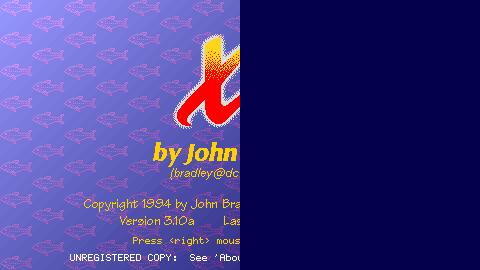
\includegraphics[width=7.0cm]{cv_kadai01/image.png}
\caption{画面左半分のみ色を変換した結果}
\label{fig:2-2-1kairo}
\end{center}
\end{figure}



